\documentclass[kulak]{kulakarticle} % options: kulak (default) or kul

\usepackage[dutch]{babel}

\title{Eindverslag teamopdracht machine learning - Team $\exists$uler}
\author{\small Daan, Marie, Zeineb, Florian, Vincent, Jasper, Lasha \& Younes}
\date{Academiejaar 2023 -- 2024}
\address{
	\textbf{Groep Wetenschap \& Technologie Kulak} \\
	Teamopdracht P\&O1 - IW}

\begin{document}

\maketitle

\section*{Inleiding}

Inleidende tekst.

\section*{Simulatie 1}

Vóór de aanvang van de sessie was simulatie 1 reeds in orde gebracht.
In deze simulatie hebben we een steekproef \((x_i, 10^{x_i} + \epsilon_i)\) van 20 punten met een standaardnormaal verdeeld residu en een uniform verdeelde regressor tussen 0 en 1. We stelden de steekproef grafisch voor, voegden de populatiefunctie toe, de regressielijn en de KNN-modellen voor \(K=1\), \(K=5\) en \(K=20\):

\begin{figure}[h!]
	\centering
	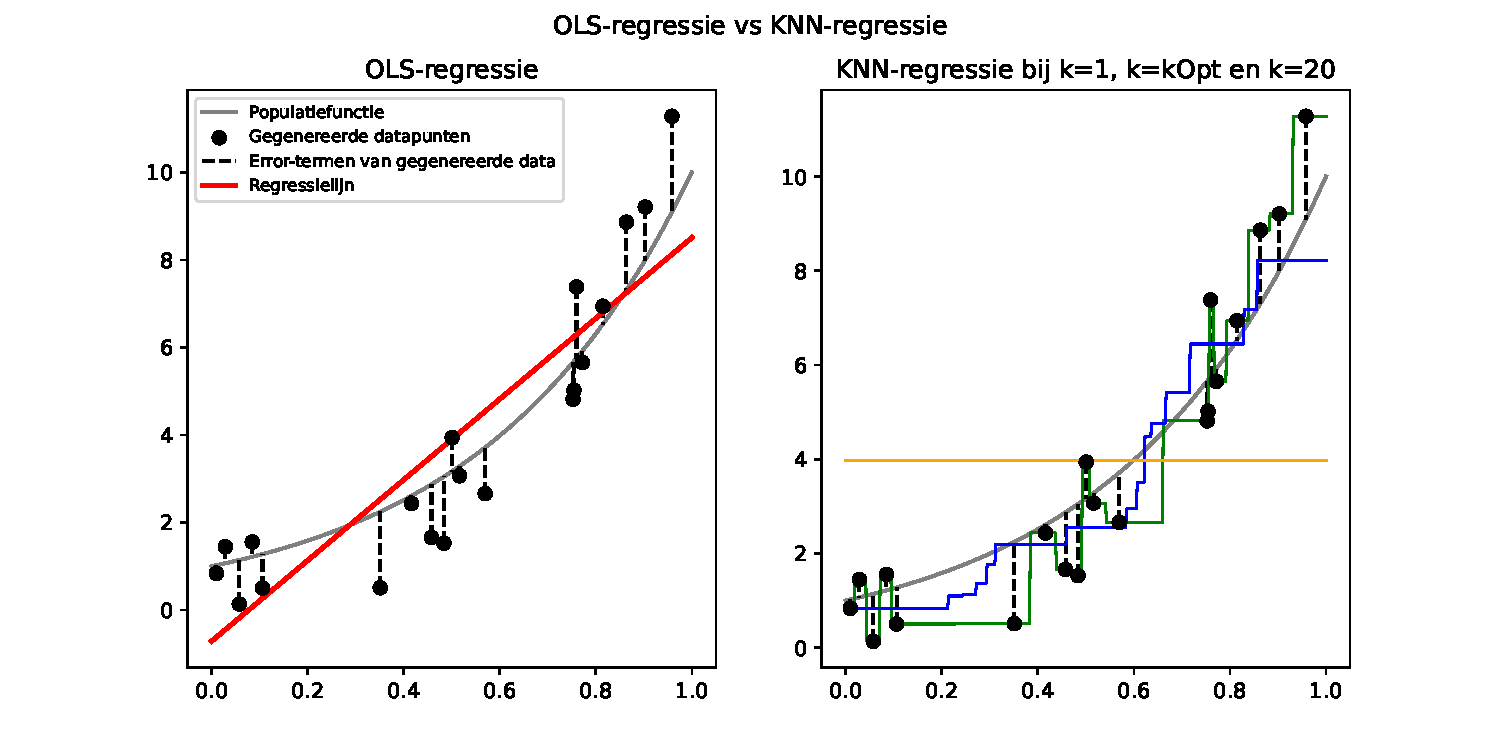
\includegraphics[width=0.8\textwidth]{simulatie1}
	\label{fig:simulatie1}
	\caption{OLS-regressie vergeleken met KNN-regressie voor verschillende waarden van \(K\).}
\end{figure}

De OLS-regressielijn is lineair, wat ervoor zorgt dat de populatiefunctie - die niet lineair is - niet super goed benaderd wordt.

Bij de (groene) KNN-regressielijn voor \(K=1\) is er duidelijk sprake van \textit{overfitting}: de regressielijn volgt elk datapunt perfect en wordt dus ook heel sterk beïnvloed door uitschieters. De (blauwe) regressielijn voor \(K=5\) heeft een lagere bias, aangezien deze regressielijn zich op de 5 dichtstbijzijnde buren baseert en dus veel minder gevoelig is voor uitschieters in de gegenereerde dataset. Wanneer \(K=20\), is de KNN-regressielijn een rechte waarvan de y-waarde gelijk is aan de gemiddelde y-waarde van alle datapunten, aangezien het aantal datapunten ook gelijk is aan 20. We besluiten dus dat de regressielijn voor \(K=5\) de beste schatter is.

\section*{Besluit}

Afsluitende tekst.

\end{document}
